\documentclass[12pt, titlepage]{article}

\usepackage{fullpage}
\usepackage[round]{natbib}
\usepackage{multirow}
\usepackage{booktabs}
\usepackage{tabularx}
\usepackage{graphicx}
\usepackage{float}
\usepackage{hyperref}
\hypersetup{
colorlinks,
citecolor=blue,
filecolor=black,
linkcolor=red,
urlcolor=blue
}
\usepackage{subfig}

%% Comments

\usepackage{color}

\newif\ifcomments\commentstrue %displays comments
%\newif\ifcomments\commentsfalse %so that comments do not display

\ifcomments
\newcommand{\authornote}[3]{\textcolor{#1}{[#3 ---#2]}}
\newcommand{\todo}[1]{\textcolor{red}{[TODO: #1]}}
\else
\newcommand{\authornote}[3]{}
\newcommand{\todo}[1]{}
\fi

\newcommand{\wss}[1]{\authornote{blue}{SS}{#1}} 
\newcommand{\plt}[1]{\authornote{magenta}{TPLT}{#1}} %For explanation of the template
\newcommand{\an}[1]{\authornote{cyan}{Author}{#1}}

%% Common Parts

\newcommand{\progname}{REVITALIZE} % PUT YOUR PROGRAM NAME HERE
\newcommand{\authname}{Team 13, REVITALIZE
\\ Bill Nguyen
\\ Syed Bokhari
\\ Hasan Kibria
\\ Youssef Dahab
\\ Logan Brown
\\ Mahmoud Anklis} % AUTHOR NAMES                  

\usepackage{hyperref}
    \hypersetup{colorlinks=true, linkcolor=blue, citecolor=blue, filecolor=blue,
                urlcolor=blue, unicode=false}
    \urlstyle{same}
                                


\newcounter{acnum}
\newcommand{\actheacnum}{AC\theacnum}
\newcommand{\acref}[1]{AC\ref{#1}}

\newcounter{ucnum}
\newcommand{\uctheucnum}{UC\theucnum}
\newcommand{\uref}[1]{UC\ref{#1}}

\newcounter{mnum}
\newcommand{\mthemnum}{M\themnum}
\newcommand{\mref}[1]{M\ref{#1}}

\begin{document}

\title{System Design for \progname{}} 
\author{\authname}
\date{\today}

\maketitle

\pagenumbering{roman}

\section{Revision History}

\begin{tabularx}{\textwidth}{p{3cm}p{2cm}X}
	\toprule {\bf Date} & {\bf Version} & {\bf Notes}\\
	\midrule
	January 18th, 2023 & Syed Bokhari & Added user interface figma sketches\\
	January 18th, 2023 & Syed Bokhari & Added interface descriptions and additional information\\
	January 18th, 2023 & Syed Bokhari & Added reflection question answers\\
	January 17th, 2023 & Mahmoud Anklis & Added introduction, purpose, and scope\\
	January 18th, 2023 & Mahmoud Anklis & Added project overview, reference material, timeline, and reflection\\
	January 18th, 2023 & Youssef Dahab & Added reflection\\
	\bottomrule
\end{tabularx}

\newpage

\section{Reference Material}

This section records information for easy reference.

\subsection{Abbreviations and Acronyms}

\renewcommand{\arraystretch}{1.2}
\begin{tabular}{l l} 
	\toprule		
	\textbf{symbol} & \textbf{description}\\
	\midrule 
	AC & Anticipated Change\\
	DAG & Directed Acyclic Graph \\
	M & Module \\
	MG & Module Guide \\
	OS & Operating System \\
	R & Requirement\\
	SC & Scientific Computing \\
	SRS & Software Requirements Specification\\
	\progname & Explanation of program name\\
	UC & Unlikely Change \\
	\bottomrule
\end{tabular}\\

\newpage

\tableofcontents

\newpage

\listoftables

\listoffigures

\newpage

\pagenumbering{arabic}

\section{Introduction}
The following document details the System Design for
the REVITALIZE app. The REVITALIZE app is an all-in-one health and wellness app, comprised of 1 main 
section and 3 major subsections. The main section is a calendar which organizes and documents the contents of the 3 subsections. 
The 3 subsections are the diet section, workout section, and sleep section.

The full documentation and implementation can be
found at \url{https://github.com/BillNguyen1999/REVITALIZE/tree/main/docs}.


\section{Purpose}

The purpose of the design documentation is to illustrate how the software application will meet the requirements. The System Design document will display the design of the interface as well as the connection between the requirements and the design of the application. 


\section{Scope}

The scope of this software application is to provide an all-in-one health app for adults/teenagers of any age. Users of REVITALIZE can track their diet, sleep, and workouts as well as find recipes for meals based on nutritional specifications. 
\begin{figure}[H]
	\centering
	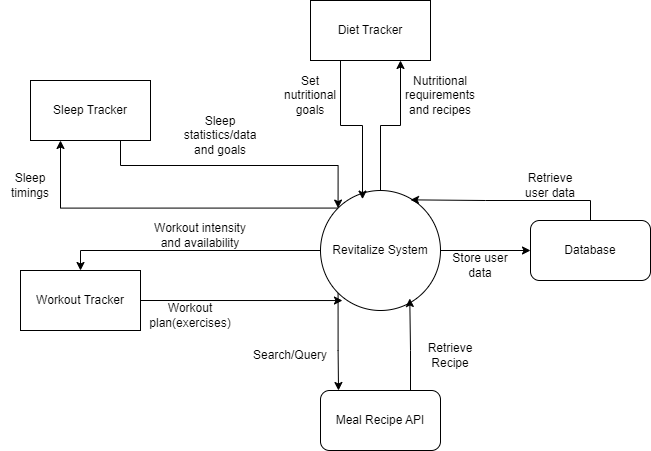
\includegraphics[scale=0.5]{system_diagrams/SystemContextDiagram.png}
	\caption{\textcolor{black} System context diagram for Revitalize}
\end{figure}


\section{Project Overview}

\subsection{Normal Behaviour}
The application is comprised of one main section and three subsections. The main section includes a calendar that can be selected and interacted with. The three subsections will allow users' to track their diet, sleep, as well as their workouts. The diet section includes a recipe finder that provides the user with a search engine for recipes of meals based on nutritional filters. The sleep section tracks the user's sleep and provides important statistics and recommendations. The workout section allows the user to plan workouts by selecting pre-existing workouts and modifying the number of sets and reps. Overall, the REVITALIZE application will help user's achieve a healthy lifestyle.

\subsection{Undesired Event Handling}

In the event that undesired events take place, the REVITALIZE application will have error handling checks to safeguard the application from failing. In the case of potential errors with user input, the system will put in place enforced type checks. For example, when the user wants to input the number of calories for a recipe search, the input will only be numerical. Additionally, in the case of a system error, the application will catch and handle that error, ensuring that the system does not fail. 

\subsection{Component Diagram}
\begin{figure}[H]
	\centering
	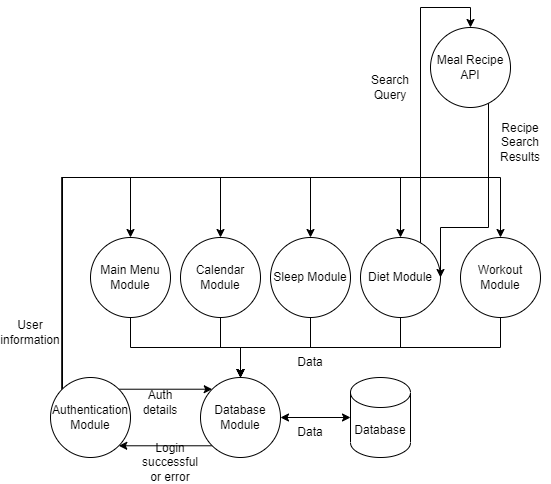
\includegraphics[scale=0.7]{system_diagrams/SystemComponentDiagram.png}
	\caption{\textcolor{black} System component diagram for Revitalize}
\end{figure}
\subsection{Connection Between Requirements and Design} \label{SecConnection}

The system design of REVITALIZE is founded upon the requirements previously set in the SRS. It is designed to cater for every single requirement attributed to this project. Hence, the design is decomposed into modular pieces of functionality which each help serve the fulfillment of aforementioned requirements. Specifications on how each module relates to (a) requirement(s) can be found in Section 8 of the MG document.\\
The functional outlook of each module can be understood by its name and, if needed, its access programs detailed in the MIS. After realizing the functionality of each module, the connections outlined in the Traceability Matrix in Section 8 of the MG document should be clear and easily comprehended.

\section{System Variables}

N/A

\subsection{Monitored Variables}
N/A
\subsection{Controlled Variables}
N/A
\subsection{Constants Variables}
N/A
\section{User Interfaces}

\begin{figure}[H]%
	\centering
	\subfloat[\centering Start]{{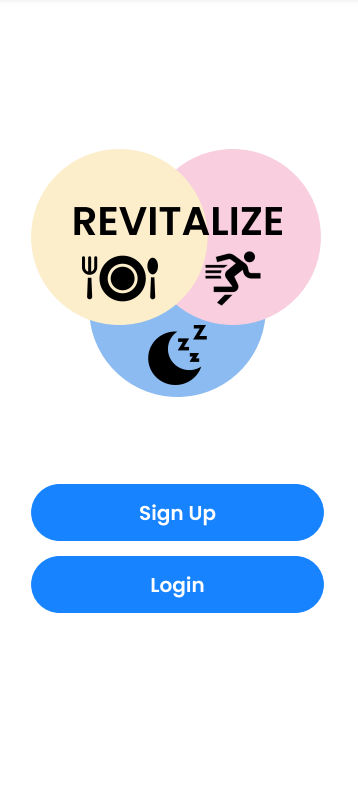
\includegraphics[width=5cm]{revitalize_figma_sketches/p1.png} }}%
	\subfloat[\centering Signup]{{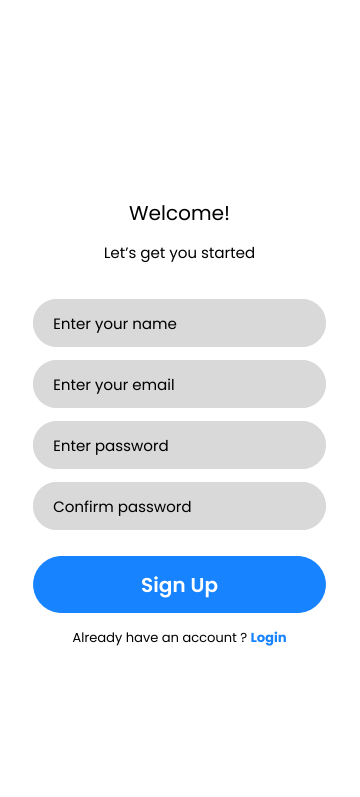
\includegraphics[width=5cm]{revitalize_figma_sketches/p2.png} }}%
	\subfloat[\centering Login]{{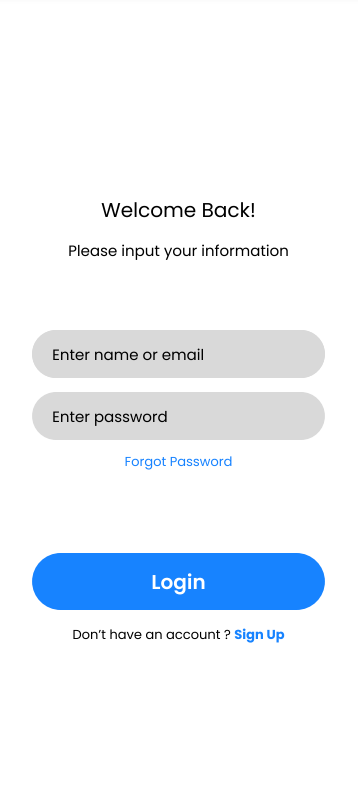
\includegraphics[width=5cm]{revitalize_figma_sketches/p3.png} }}%
	\label{fig:example}%
\end{figure}

\begin{figure}[H]%
	\centering
	\subfloat[\centering Main]{{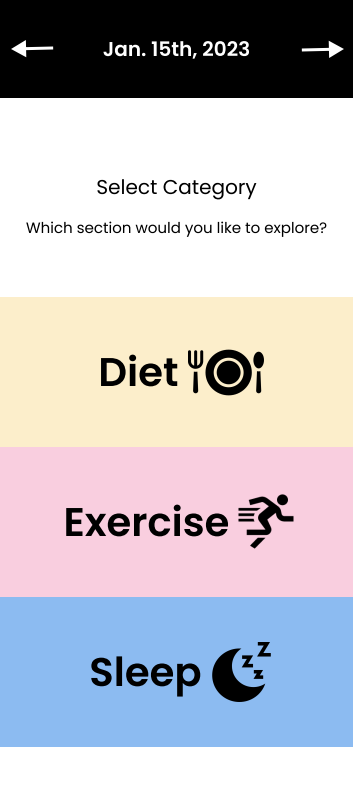
\includegraphics[width=5cm]{revitalize_figma_sketches/p4.png} }}%
	\subfloat[\centering Diet Main]{{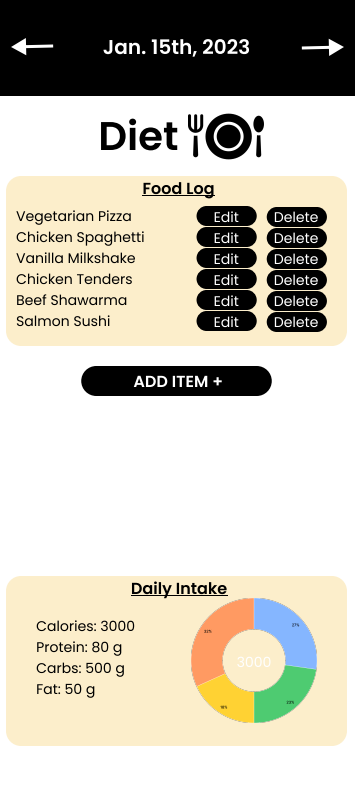
\includegraphics[width=5cm]{revitalize_figma_sketches/p5.png} }}%
	\subfloat[\centering Diet Search/Add Custom Meal]{{
\includegraphics[width=5cm]{revitalize_figma_sketches/p6.png} }}%
	\label{fig:example}%
\end{figure}

\begin{figure}[H]%
	\centering
	\subfloat[\centering Diet Add Custom Meal]{{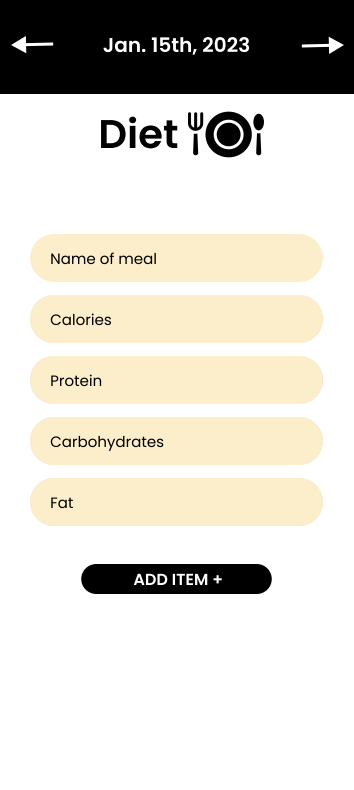
\includegraphics[width=5cm]{revitalize_figma_sketches/p7.png} }}%
	\subfloat[\centering Diet Recipe Search]{{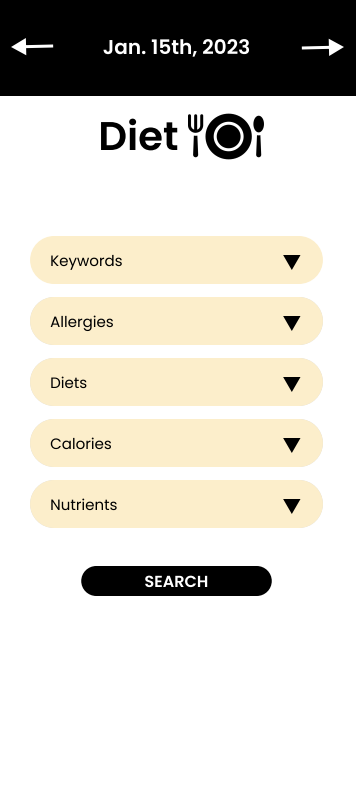
\includegraphics[width=5cm]{revitalize_figma_sketches/p8.png} }}%
	\subfloat[\centering Diet Recipe List]{{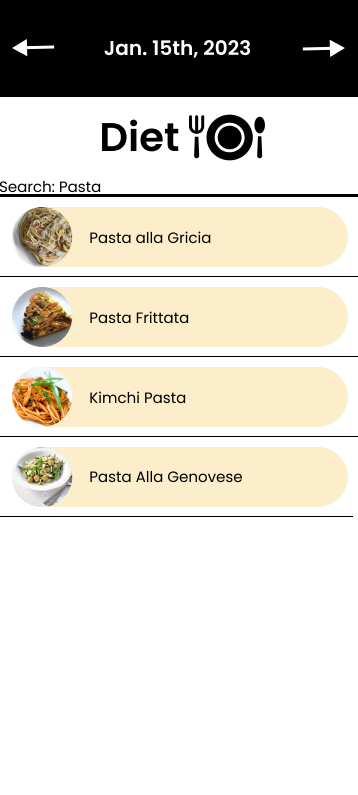
\includegraphics[width=5cm]{revitalize_figma_sketches/p9.png} }}%
	\label{fig:example}%
\end{figure}

\begin{figure}[H]%
	\centering
	\subfloat[\centering Diet Recipe Info]{{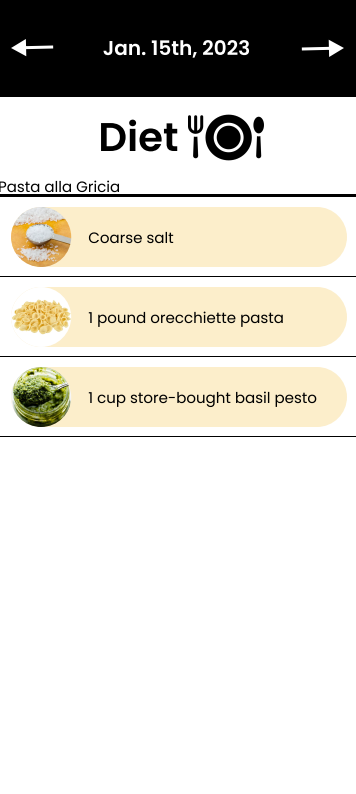
\includegraphics[width=5cm]{revitalize_figma_sketches/p10.png} }}%
	\subfloat[\centering Exercise Main]{{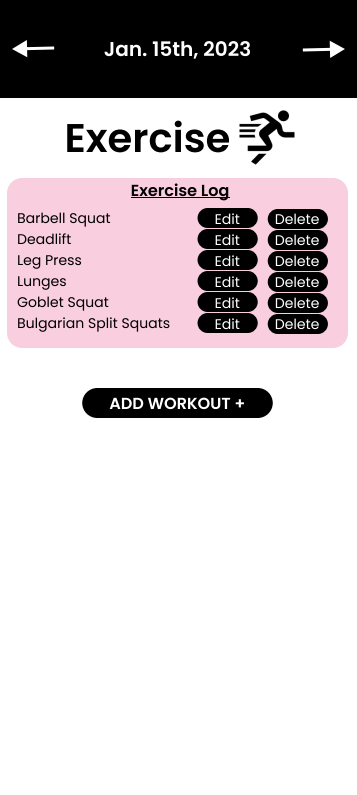
\includegraphics[width=5cm]{revitalize_figma_sketches/p11.png} }}%
	\subfloat[\centering Exercise List]{{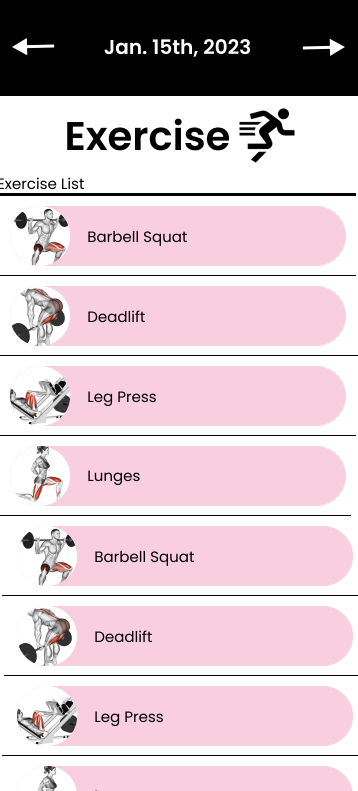
\includegraphics[width=5cm]{revitalize_figma_sketches/p12.png} }}%
	\label{fig:example}%
\end{figure}

\begin{figure}[H]%
	\centering
	\subfloat[\centering Exercuse Details]{{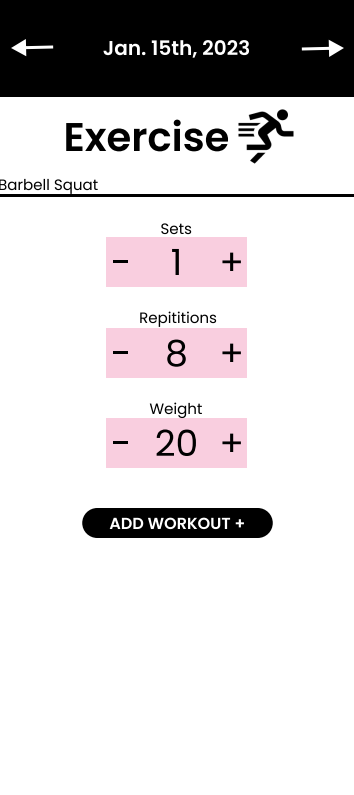
\includegraphics[width=5cm]{revitalize_figma_sketches/p13.png} }}%
	\subfloat[\centering Sleep]{{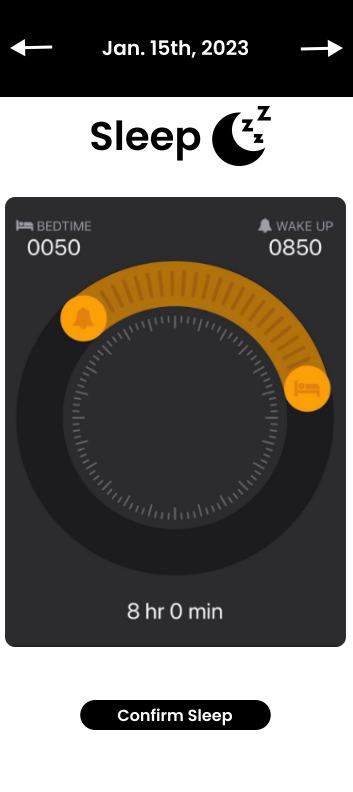
\includegraphics[width=5cm]{revitalize_figma_sketches/p14.png} }}%
	\label{fig:example}%
\end{figure}


\section{Design of Hardware}

N/A

\section{Design of Electrical Components}

N/A

\section{Design of Communication Protocols}

N/A

\section{Timeline}

\begin{table}[H]
	\begin{tabular}{|l|l|l|l|}
		\hline
		Figure & Timeline Rev 0   & Timeline Final Rev & Who's Responsible           \\ \hline
		a      & February 6, 2023 & March 20, 2023     & Logan and Youssef           \\ \hline
		b      & February 6, 2023 & March 20, 2023     & Logan and Mahmoud           \\ \hline
		c      & February 6, 2023 & March 20, 2023     & Logan and Mahmoud           \\ \hline
		d      & February 6, 2023 & March 20, 2023     & Bill and Faiq               \\ \hline
		e      & February 6, 2023 & March 20, 2023     & Faiq and Hasan              \\ \hline
		f      & February 6, 2023 & March 20, 2023     & Faiq and Hasan              \\ \hline
		g      & February 6, 2023 & March 20, 2023     & Faiq and Mahmoud            \\ \hline
		h      & February 6, 2023 & March 20, 2023     & Youssef, Mahmoud, and Hasan \\ \hline
		i      & February 6, 2023 & March 20, 2023     & Youssef, Mahmoud, and Hasan \\ \hline
		j      & February 6, 2023 & March 20, 2023     & Youssef, Mahmoud, and Hasan \\ \hline
		k      & February 6, 2023 & March 20, 2023     & Bill and Logan              \\ \hline
		l      & February 6, 2023 & March 20, 2023     & Bill and Logan              \\ \hline
		m      & February 6, 2023 & March 20, 2023     & Bill and Logan              \\ \hline
		n      & February 6, 2023 & March 20, 2023     & Bill and Youssef            \\ \hline
	\end{tabular}
\end{table}

% \bibliographystyle {plainnat}
% \bibliography{../../../refs/References}

\newpage{}

\appendix

\section{Interface}

figure (a): This is the start screen when launching the application. It offers the user the ability to either sign up or login.
\\figure (b): This is the signup screen. The user must input valid information and register with confirmation from the database.
\\figure (c): This is the login screen. The user must input valid credentials to successfully enter the main screen.
\\figure (d): This is the main screen. The user can select from the three application categories and enter their specific page after click. The user can select the calender value and change the date accordingly to see the information for the given day.
\\figure (e): This is the diet main screen. The food log is available to view and each entry can be edited or deleted. On the bottom of the screen, the total statistics of the day can be seen. The add item button is clicked to go to figure (f).
\\figure (f): This is the screen to traverse to the search or add custom meal pages.
\\figure (g): This is the custom meal screen. The user can input custom information to add to the food log.
\\figure (h): This is the recipe search screen. The user can select the API query options from the drop down to construct a unique recipe list.
\\figure (i): This is the recipe list screen. The recipes are listed based on the previous page query. 
\\figure (j): This is the recipe information screen. Specific information relating to incredients for each recipe is listed.
\\figure (k): This is the exercise main screen. It displays a list of exercises for the day that can be edited or deleted. A workout can be added by clicking the button.
\\figure (l): This is the exercise list screen.The screen displays a list of exercises available through the API. Once selected, the user is taken to figure m where they can add the custom information for their exercise. 
\\figure (m): This is the execise details screen. The user can customize their sets, reps and weight for accurate tracking.
\\figure (n): This is the sleep screen. The user can alter the clock value if the API sleep tracking was not correct and they can confirm the entry to add to their sleep log. 

\section{Mechanical Hardware}
N/A
\section{Electrical Components}
N/A
\section{Communication Protocols}
N/A
\section{Reflection}

The information in this section will be used to evaluate the team members on the
graduate attribute of Problem Analysis and Design.  Please answer the following questions:

\begin{enumerate}
	\item What are the limitations of your solution?  Put another way, given
	unlimited resources, what could you do to make the project better? (LO\_ProbSolutions)
	
	\textbf{Syed}: Our main features are reliant on the database provided by external APIs. The recipe list and the exercise list can only give the user's the information that is accessable through the API. This limits the design of the app due to the limited query information. \\
	\textbf{Bill}: Project does not have functionalities such as analytics of data and predictive models that can potentially benefit the user experience. \\
	\textbf{Hasan}: Since time is a key resource, unlimited resources would imply unlimited time. I think with unlimited (or rather plenty of) time, we could improve every aspect- from the documentation to the UI to the business logic. \\
	\textbf{Youssef}: Another limitation is that since a lot of REVITALIZE's features rely on making API calls, an internet connection is required for the app to work. \\
	\textbf{Mahmoud:} We can make the project better by linking the application with hardware that measures a user's heart rate and oxygen levels during their sleep. This can be extremely beneficial for a person with sleep apnea, for example, as vital sleep information can be tracked and stored.
	
	
	
	\item Give a brief overview of other design solutions you considered.  What
	are the benefits and tradeoffs of those other designs compared with the chosen
	design?  From all the potential options, why did you select documented design?
	(LO\_Explores)
	
	\textbf{Syed}: We considered a self serving exercise list, where the user would be able to add their own custom exercises. This seemed like a great option for user customizability, however the tradeoff is that the user must spend a tedious amount of time inputting the information. Instead, we have a preset list of the most common exercises that the user can quickly select and add their sets, repetitions and weight. \\
	\textbf{Bill}: We considered using analytics to find statistics and trends of which features are used the most/the least etc. which could help us improve user experience. Also considered using predictive models such as giving recipe/exercise suggestions to user based on user data. These were great options, but are options that are nice to have and were considered stretch goals. \\
	\textbf{Hasan}: To be honest I do not completely remember all the other design solutions we covered. However, I do remember that this design solution stood out because it solved a real problem; ie. an all-in-one health application that is user friendly and easily learned. \\
	\textbf{Mahmoud:} We had other design solutions for the way to match meals, exercise, and sleep with each day. We decided to go with a main calendar design because of its simplicity and ease of access. \\
	\textbf{Youssef:} Another design solution we considered was sending users notifications to remind them to workout or view their nutritional intake that they should follow. This idea was an on shelf stretch goal.
\end{enumerate}

\end{document}